
%!TEX ROOT=main.tex


\part{Software}
\label{chap:software}
\section{Introduction}
The control program for both the transmitter and the car is written in C language. It utilizes the STM32 HAL (Hardware Abstraction Layer) libraries, and the STM32CubeMX graphical utility was used to set up the necessary initialization and project files and generate code for peripheral configuration.

STM32 HAL driver library provides a set of APIs to simplify interaction with all the peripherals and thus the user application implementation. The HAL driver layer implements run-time failure detection to increase robustness. HAL APIs are available for all peripherals. Also, the API ensures high portability across different STM32 families \cite{hal}.

STM32CubeMX is a graphical tool that provides a convenient user interface to configure the microcontroller. It allows a simple configuration of pin assignments, peripherals, or the clock tree, and the corresponding C initialization code generation. It also packs middleware stacks, such as USB, FatFs, or TCP/IP. This tool notably speeds up the process of microcontroller configuration and allows the user to focus on the application \cite{cubemx}.

The control program is almost exclusively interrupt-driven. Emphasis has been placed on program execution speed to ensure a high frequency of control commands and, therefore, smooth car control.

\section{Transmitter}
\subsection{Peripherals and pin configuration}
\begin{figure}[t]
\centering
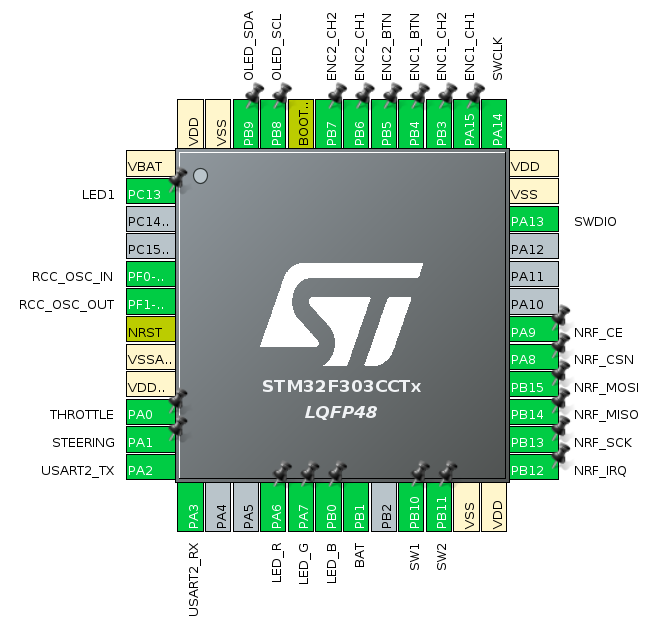
\includegraphics[width=0.7\linewidth]{fig/tx_pin_assignments.png}
\caption{Transmitter pin assignments}
\label{fig:tx_conf}
\end{figure}
The microcontroller runs at \SI{72}{\MHz} with a clock source set to a \SI{12}{\MHz} external crystal oscillator.

ADC1 channels 1 and 2 are used to measure the output voltage from control potentiometers. ADC operates with 12-bit resolution in continuous conversion mode with DMA enabled in circular mode with continuous requests to manipulate the data. Once the ADC conversion is started, it remains active, and DMA repeatedly fills the buffer with measured data. Sampling time is the highest possible 601.5 cycles to acquire stable measurements.

ADC3 uses channel 1 to measure the LiPo battery voltage and channel Vrefint to measure the internal reference voltage. Again, the resolution is 12-bit, continuous conversion mode is enabled, and DMA is utilized to transfer data from peripheral to memory. In this mode, the ADC remains active until DMA fills the whole data buffer. The sampling time for channel 1 is $601.5$ cycles, and for channel Vrefint $181.5$ cycles.

The communication module is connected to the SPI2 bus operating in full-duplex master mode. Baud rate is set to \SI{9}{\mega\bit\per\second}, and the data size is standard 8 bits. 'NRF\_IRQ' pin is configured in external interrupt mode with rising edge detection. The rest of the 'NRF' pins are simple outputs.

Quadrature rotary encoders utilize timers TIM2 and TIM4, which are in Encoder mode. This mode is designed specially to interface quadrature encoders with out-of-phase output signals. Encoder push-button pins are configured in external interrupt mode with rising edge detection.

SW1 and SW2 pins belong to the DIP switch and are configured in external interrupt mode with both rising and falling edge detection.

USART2 peripheral is configured as debug serial port. Baud rate is set to \SI{921600}{\bit\per\second} with 8 bits word length and one stop bit.

I2C1 in Fast Mode Plus with a frequency of \SI{1}{\MHz} connects the OLED display, and LED pins are simple outputs. Figure \ref{fig:tx_conf} shows the complete pinout in STM32CubeMX.





\section{Car}
\subsection{Peripherals and pin configuration}
\begin{figure}[t]
\centering
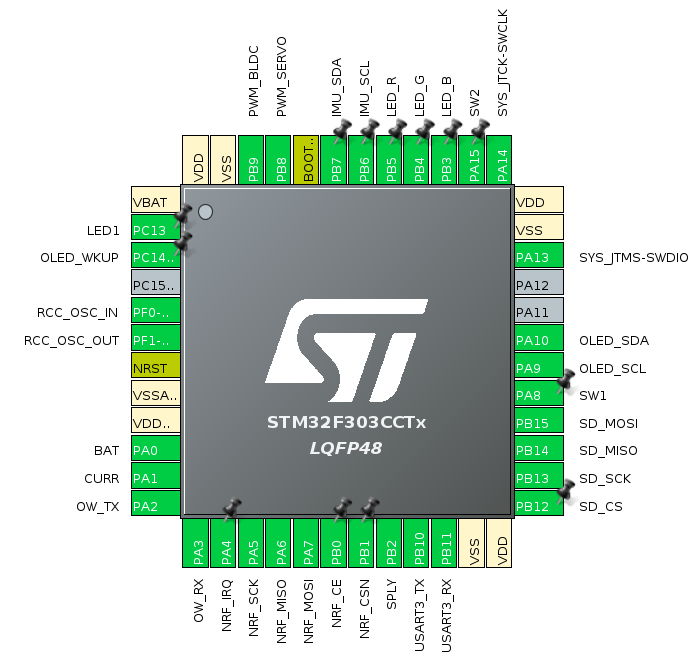
\includegraphics[width=0.75\linewidth]{fig/car_pin_assignments.png}
\caption{Car pin assignments}
\label{fig:car_conf}
\end{figure}
Some of the settings are similar to transmitter settings since both microcontrollers are the same STM32F303CCT6. The microcontroller runs at \SI{72}{\MHz} with a clock source set to an \SI{8}{\MHz} external crystal oscillator.

Channels 2 and 3 of timer TIM8 are used to generate PWM and therefore control the car. Prescaler and counter period values are calculated to represent the pulse width in microseconds. That means the counter value of e.g. $1500$ equals \SI{1500}{\micro\second} pulse width, which is convenient for control application implementation.

ADC1 channels 1 and 2 are used to measure the LiPo battery voltage and output voltage from the current sensor. ADC operates with 12-bit resolution in continuous conversion mode with DMA enabled. Sampling time is again the highest possible $601.5$ cycles to acquire stable measurements.

ADC2 measures the Vrefint channel to obtain the internal reference voltage and channel 12 to obtain the BEC output voltage. The resolution is also 12-bit, and continuous conversion mode with DMA is enabled. The sampling time for channel Vrefint is $181.5$ cycles and $601.5$ cycles for channel 12.

The communication module is connected to the SPI1 bus operating in full-duplex master mode. Baud rate is set to \SI{9}{\mega\bit\per\second}, and the data size is standard 8 bits. 'NRF\_IRQ' pin is configured in external interrupt mode with rising edge detection. The rest of the 'NRF' pins are simple outputs.

As STM32F303 does not support the SDIO interface, the SD card is connected via the SPI2 peripheral. The baud rate is only \SI{281.25}{\kilo\bit\per\second} after reset, but once the SD card is initialized, it is increased to \SI{9}{\mega\bit\per\second}.

I2C2 in Fast Mode Plus with a frequency of \SI{1}{\MHz} connects the OLED display. IMU unit is served by I2C1 in Fast Mode with a frequency of \SI{400}{\kHz}.

1-Wire bus necessary to communicate with the DS18B20 temperature sensor is implemented using USART2 peripheral and DMA. The implementation is described in section *sec*. [\todo section]

SW1 and SW2 pins belong to the DIP switch and are configured in external interrupt mode with both rising and falling edge detection.

USART3 peripheral is configured as debug serial port. Baud rate is set to \SI{921600}{\bit\per\second} with 8~bits word length and one stop bit.

LED pins are simple outputs. Pins PA11 and PA12 are not used in the project's current state but are reserved for USB peripherals for possible future expansion with a control computer.

Figure \ref{fig:car_conf} shows the complete pinout in STM32CubeMX.